\section{Introduction}

\begin{frame}
\frametitle{Roadmap}
\begin{center}
\begin{enumerate}
\item Binders and Linearity
\begin{itemize}
\item[\textbf{Act I}:] Binary Session Types
\end{itemize}
\item Multiparty Processes and Coinduction
  \begin{itemize}
  \item[\textbf{Act II}:] Mechanising Multiparty Processes
  \item[\textbf{Act III}:] Mechanising Multiparty Session Types
  \end{itemize}
\end{enumerate}
\end{center}
\end{frame}


% not the standard notion of binders because they have operational meaning
%
\begin{frame}
\frametitle{SmolEMTST: Tutorial Repository}
  \begin{picture}(0,0)
    {
        \put(70,-90){%\begin{shbox}{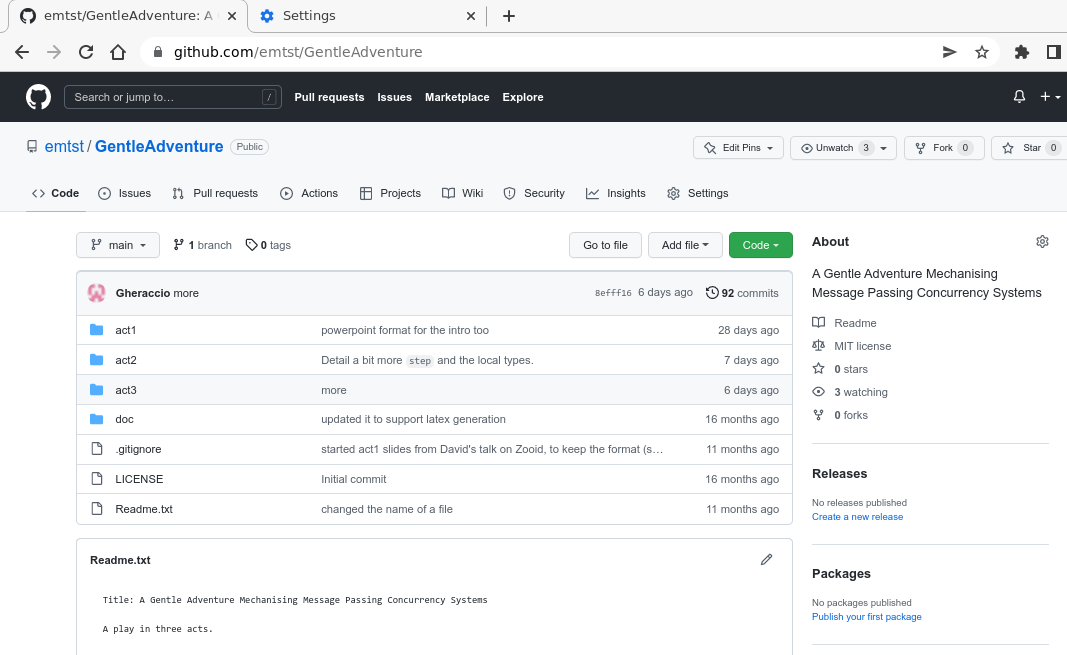
\includegraphics[width=1.1\textheight]{figures/smolZooid.png}}\end{shbox}
\begin{tcolorbox}[beamer,
                  width=1.1\textheight,
                  arc=0pt,
                  boxsep=0pt,
                  left=0pt,right=0pt,top=0pt,bottom=0pt,
                  ]
    \includegraphics[width=\linewidth]{figures/smolzooid.png}
\end{tcolorbox}
}
        \put(100,-95){% \only<2->{\shadowbox{
\includegraphics[width=.9\textheight]{figures/emtst-paper.png}}}
\only<2->{%
\begin{tcolorbox}[beamer,
                  width=.9\textheight,
                  arc=0pt,
                  boxsep=0pt,
                  left=0pt,right=0pt,top=0pt,bottom=0pt,
                  ]
    
\includegraphics[width=\linewidth]{figures/emtst-paper.png}
\end{tcolorbox}
}
}
        \put(60,-40){%\only<3->{\shadowbox{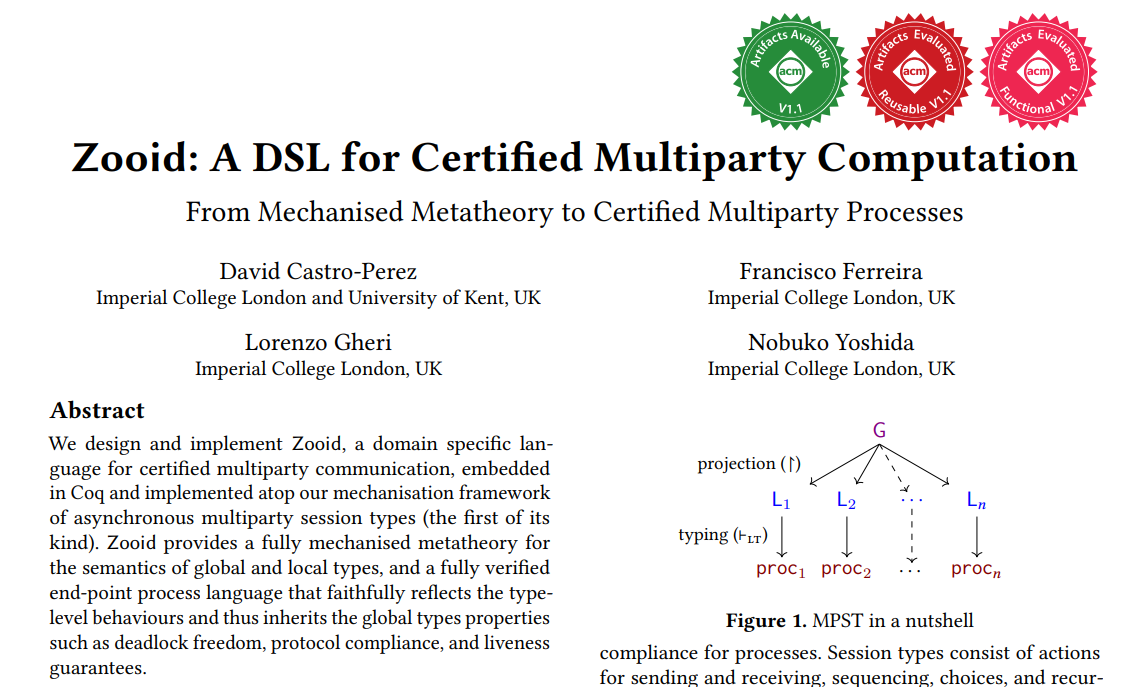
\includegraphics[width=.9\textheight]{figures/cmpst-paper.png}}}
\only<3->{%
\begin{tcolorbox}[beamer,
                  width=.9\textheight,
                  arc=0pt,
                  boxsep=0pt,
                  left=0pt,right=0pt,top=0pt,bottom=0pt,
                  ]
    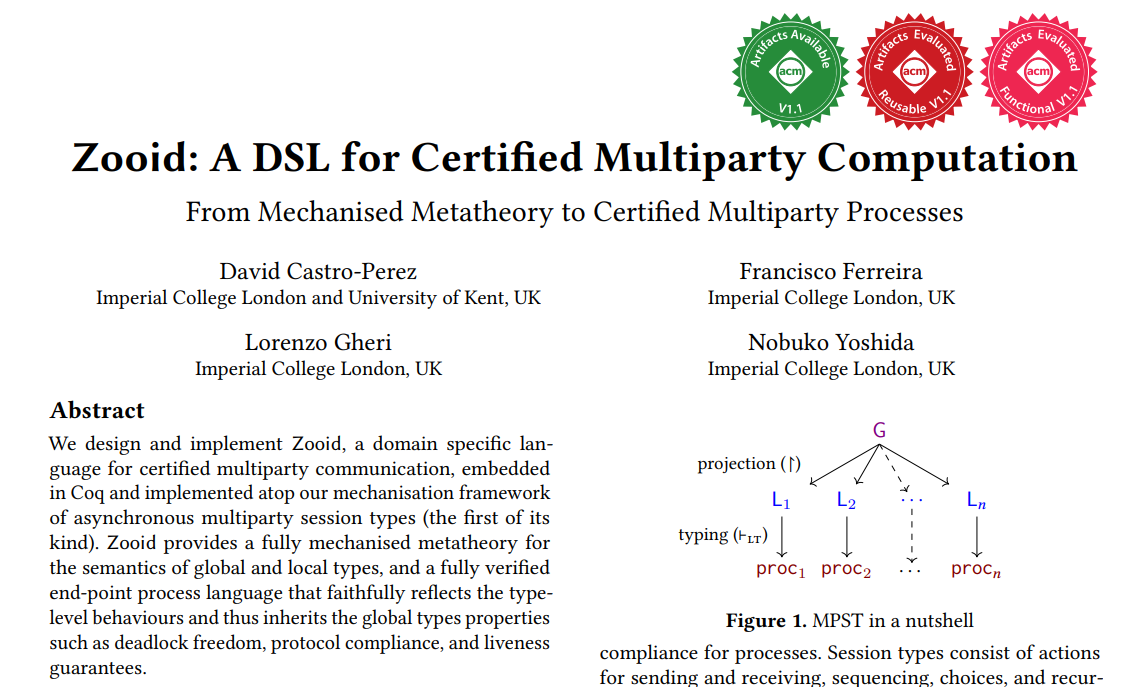
\includegraphics[width=\linewidth]{figures/cmpst-paper.png}
\end{tcolorbox}
}
}
    }
  \end{picture}
\end{frame}
